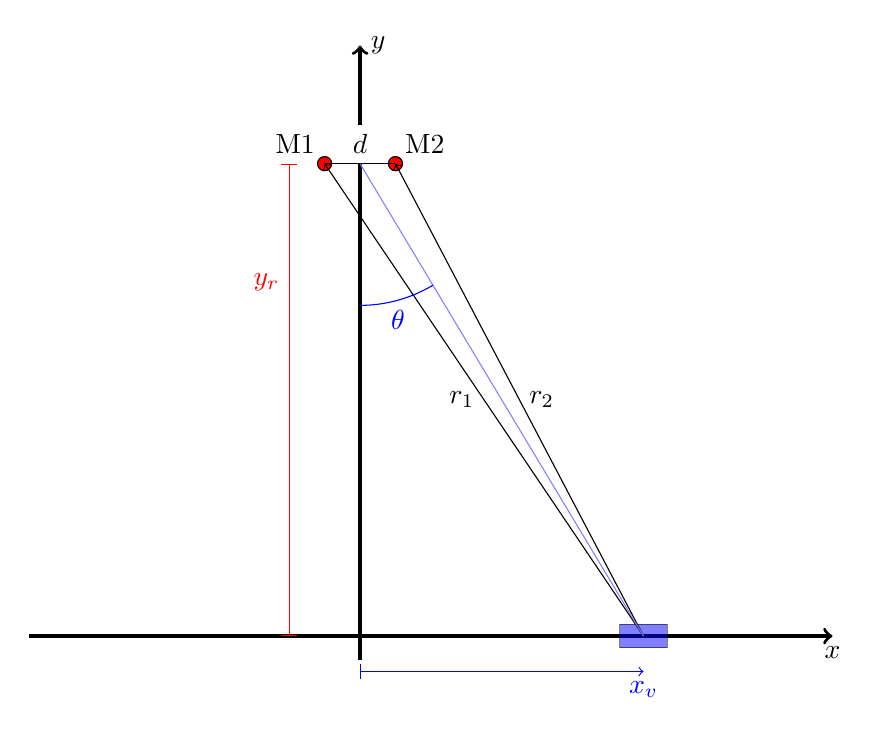
\begin{tikzpicture}[scale=3][>=stealth]

	\def\angle{59}
	\def\ymax{2.5}
	\def\xmax{2.0}
	\def\yr{2.0}
	\def\xv{1.2}
	\def\d{0.3}
	\def\sourcesize{0.03}
	
	% Colours
	\colorlet{anglecolor}{blue} 
	\colorlet{roadcolor}{gray!20!black} 
	\colorlet{ycolor}{red} 
	\colorlet{xcolor}{blue}
	
	% Styles  
	\tikzstyle{axisline}=[very thick] 
	
	% Axes and road
	%\filldraw[fill=roadcolor, draw=black, nearly transparent] (-\xmax/2, -0.02) rectangle (\xmax*0.9, +0.02);
	\draw[axisline, ->] (-\xmax*0.7, 0) -- (\xmax, 0)  node[below]{$x$};
	\draw[axisline, ->] (0, -0.1) -- (0, \ymax)  node[right]{$y$};
	\filldraw[fill=xcolor, draw=black, semitransparent] (\xv-0.1, -0.05) rectangle  ++(0.2, 0.1) ;
	
	% Microphones
	\filldraw[fill=ycolor, draw=black] (-\d/2, \yr) coordinate(M1) circle (\sourcesize);
	\filldraw[fill=ycolor, draw=black] (\d/2, \yr) coordinate(M2) circle (\sourcesize);

	% Sound paths
	\draw[->] (\xv, 0) -- (M1) node[above left]{M1}  node[midway, anchor=east]{$r_1$};
	\draw[->] (\xv, 0) -- (M2) node[above right]{M2} node[midway, anchor=west]{$r_2$};;
	\draw[-, anglecolor!50!white] (\xv, 0) -- (0,\yr);
	\draw[- ] (M1) -- node[above, fill=white!] {$d$} (M2);
		
	\draw[draw=anglecolor] (0,\yr)++(0, -0.6)  arc(-90:-59:0.6) coordinate(ARC) 
		node[midway, below, anglecolor]{$\theta$};

	% Rulesr
	\draw[|->, xcolor] (0, -0.15) -- ++(\xv, 0) node[at end, below]{$x_v$};
	\draw[|-|, ycolor] (-0.3, 0) -- ++(0, \yr) node[near end, left]{$y_r$};

\end{tikzpicture}

